\definecolor{ttqqcc}{rgb}{0.33,0.33,0.33}
%dash pattern=on 5pt off 2pt
%[fill = white, rounded corners = 4pt, inner sep = 1pt]
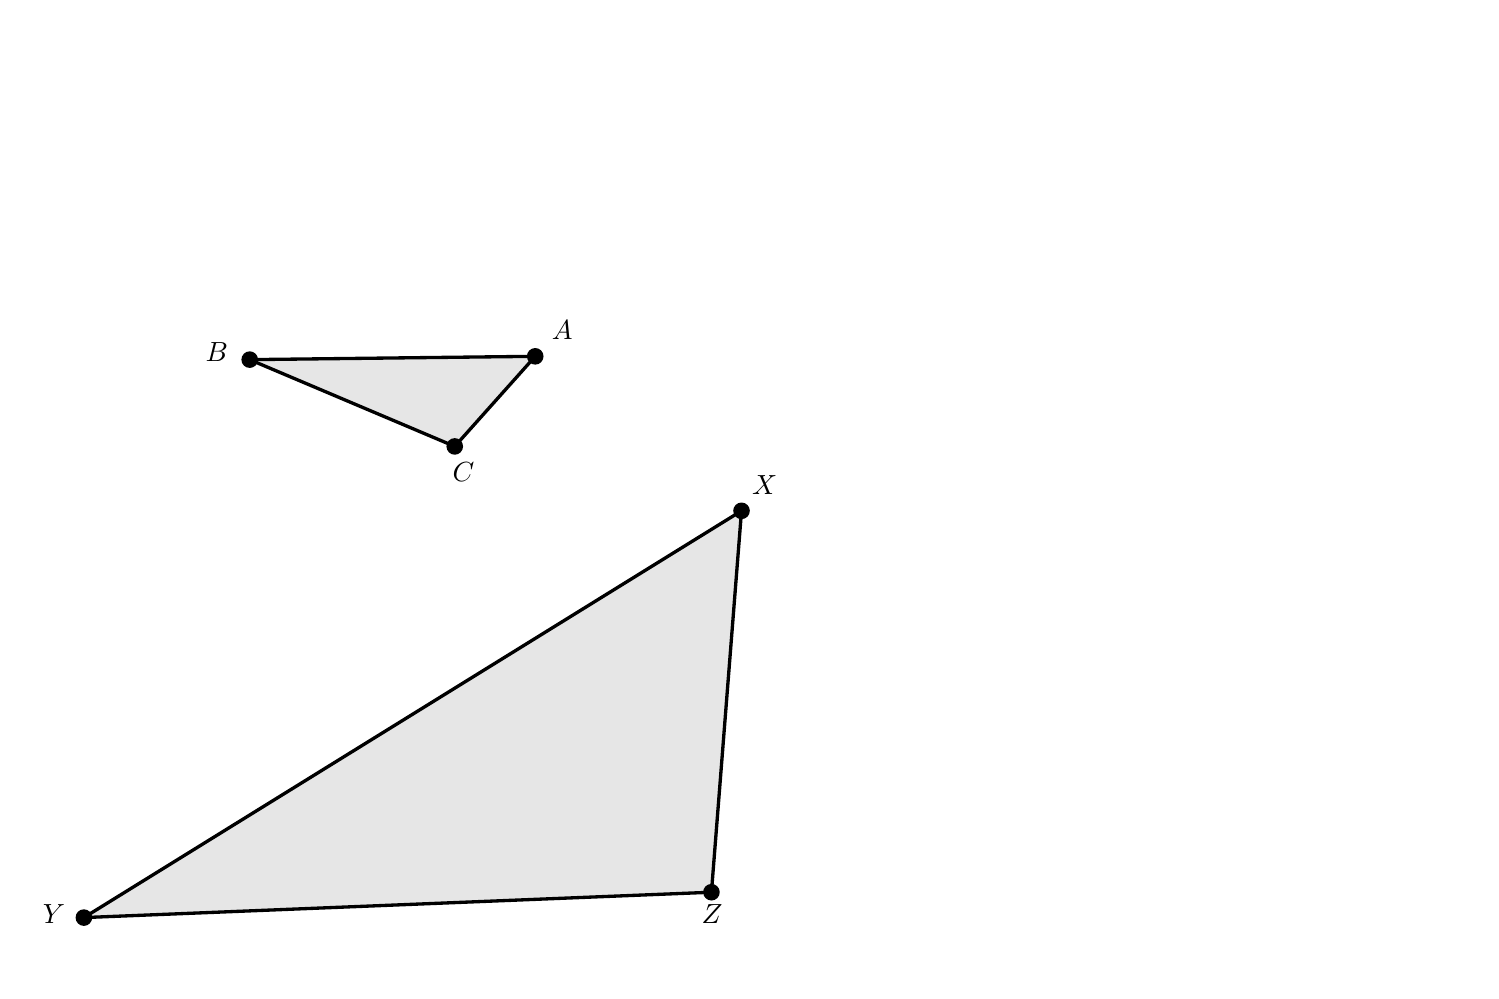
\begin{tikzpicture}[scale = 0.2]
    \clip(-25.62,-26.27) rectangle (66,33.59);
    \fill[line width=0pt,color=ttqqcc,fill=ttqqcc,fill opacity=0.15] (6.61,12.72) -- (-11.52,12.51) -- (1.5,7) -- cycle;
    \fill[line width=0pt,color=ttqqcc,fill=ttqqcc,fill opacity=0.15] (19.71,2.91) -- (-22.05,-22.92) -- (17.8,-21.31) -- cycle;
    \draw [line width=1.2pt] (6.61,12.72)-- (-11.52,12.51);
    \draw [line width=1.2pt] (-11.52,12.51)-- (1.5,7);
    \draw [line width=1.2pt] (1.5,7)-- (6.61,12.72);
    \draw [line width=1.2pt] (19.71,2.91)-- (-22.05,-22.92);
    \draw [line width=1.2pt] (-22.05,-22.92)-- (17.8,-21.31);
    \draw [line width=1.2pt] (17.8,-21.31)-- (19.71,2.91);
    \begin{scriptsize}
        \normalsize
        \fill [color=black] (-11.52,12.51) circle (15pt);
        \draw[color=black] (-13.61,13.01) node {$B$};
        \fill [color=black] (1.5,7) circle (15pt);
        \draw[color=black] (2.06,5.38) node {$C$};
        \fill [color=black] (6.61,12.72) circle (15pt);
        \draw[color=black] (8.33,14.37) node {$A$};
        \fill [color=black] (19.71,2.91) circle (15pt);
        \draw[color=black] (21.18,4.55) node {$X$};
        \fill [color=black] (-22.05,-22.92) circle (15pt);
        \draw[color=black] (-23.95,-22.72) node {$Y$};
        \fill [color=black] (17.8,-21.31) circle (15pt);
        \draw[color=black] (17.84,-22.72) node {$Z$};
    \end{scriptsize}
\end{tikzpicture}